\documentclass{article}
\usepackage{standalone}
\usepackage{multirow}
\usepackage{booktabs}
\begin{document}
  \section{Simulation und Ergebnisse} % (fold)
  \label{sec:simulation_und_ergebnisse}

    Wie in den vorherigen Abschnitten gezeigt wurde, ist es möglich, eine Finite-Elemente-Methode sowohl auf der CPU als auch auf der GPU zu implementieren.
    Der dafür erforderliche Aufwand ist annähernd vergleichbar und ist durch die Verwendung von externen Bibliotheken, wie zum Beispiel CUSP, optimierbar.
    Die Entscheidung, welche der beiden Prozessorarten besser für ein solches Problem geeignet ist, kann anhand diverser Parameter getroffen werden.
    Einer der aussagekräftigsten Parameter hierzu ist die Performance des Programms.

    In Tabelle TABELLE werden diesbezüglich unter anderem die Zeiten für die Berechnung eines Zeitschrittes der beiden Prozessorarten für verschiedene Szenengrößen verglichen.
    Dabei wurde festgestellt, dass die Implementierung auf der GPU für die betrachteten Modelle eine schnellere Berechnung ermöglicht im Vergleich zur CPU.
    Dies basiert im Wesentlichen auf der hohen Datenparallelität und der Möglichkeit der GPU, diese durch ihre extrem hohe Anzahl an Kernen auszunutzen.
    Zudem wurde die vollständige Auslastung der GPU erst für Szenen mit circa einer Million Eckpunkte und mehr erreicht.
    Dies bedeutet wiederum, dass die GPU für kleine Modelle nicht ausgelastet ist, und eine parallelisierte Implementierung auf CPU das Problem unter Umständen effizienter lösen könnte.
    Im Diagramm XY ist der Effizienzgewinn (engl.: \textit{speed up}) der GPU im vergleichbar zur CPU noch einmal dargestellt.

    Tabelle TABELLE zeigt weiterhin die Zeit, die benötigt wird, um die Systemmatrizen auf der CPU zu konstruieren.
    Der Zusammenhang zwischen Szenengröße und Konstruktionsdauer zeigt eine positive Korrelation.
    Je feiner die Auflösung des Berechnungsgebietes, desto größer wird die benötigte Konstruktionszeit.
    Diese simple Aussage ist der Tatsache geschuldet, dass die Konstruktion der Systemmatrizen auf der CPU nur seriell vollzogen wurde.
    Ein vergleichbarer Zusammenhang auf der GPU ist anhand der Messwerte nicht ersichtlich.

    Ein Vergleich der Konstruktionsdauer mit der Dauer der Zeitschrittberechnung auf der CPU zeigt, dass die Generierung der Systemmatrizen für große Modelle circa dreimal länger benötigt als die Berechnung des Zeitschrittes.
    Kleinere Systeme weisen ein noch ungünstigeres Verhältnis auf, sodass die Konstruktion sogar bis 95\% der Gesamtrechenzeit einnimmt.
    Dies stellt allerdings kein großes Problem dar, weil die Berechnung eines einzelnen Zeitschrittes beliebig oft wiederholt wird, während die Konstruktion nur einmalig ausgeführt wird.

    Die ausgewählten numerischen Methoden, wie die Diskretisierung der Funktionenräume durch Hutfunktionen, das Speichern dünnbesetzter Matrizen im CSR-Format und das iterative Lösen des linearen Gleichungssystems durch Conjugate Gradient, stellen nur eine Möglichkeit für die Implementierung einer Finite-Elemente-Methode dar.
    Dennoch zeigt sich, dass die Wahl dieser Methoden für die Simulation der Wellengleichung nicht nur ausreichend, sondern auch effizient waren.
    Gerade bei den hier betrachteten zweidimensionalen Problemen stellen die Hutfunktionen die einfachste Form der Approximation dar und sind aus diesem Grund am schnellsten zu berechnen.
    Für dünnbesetzte Matrizen existiert zwar eine Vielzahl von Speicherformaten, jedoch ist das verwendete CSR-Format eine der kompaktesten und einfachsten Varianten.
    Die Effizienz der zugrundeliegenden Datenstruktur ist nicht von dem Muster der dünnbesetzten Matrix abhängig und liefert demzufolge eine konstante Performance für unterschiedliche Szenen.
    Auch für die Lösung von linearen Gleichungssystemen existiert eine Vielzahl von Algorithmen.
    Die hier verwendete Methode zeichnet sich durch ihren iterativen Charakter aus.
    Sie benötigt während der Berechnung nur einen moderaten Speicherplatz und löst auch sehr große Systeme im zwei- und dreidimensionalen effizient unabhängig von der Permutation der Eckpunkte.
    Die Systemmatrizen sind positiv definit und symmetrisch.
    Das Verfahren nutzt diese Eigenschaften aus, um in wenigen Schritten zu einer Lösung zu gelangen.
    Des Weiteren lässt es sich durch sogenannte Vorkonditionierer verbessern.

    Jede hier beschriebene Methode wurde anhand der Wellengleichung implementiert.
    Die Behandlung der Wellengleichung kann auf weitere partielle Differentialgleichungen übertragen werden, sodass dies keine Einschränkung darstellt.
    Zu beachten ist dabei, dass die Genauigkeit der numerischen Approximation maßgeblich durch die Wahl des zugrundeliegenden Gitters und des Zeitschrittverfahrens beeinflusst wird.
    Bekannte Symmetrieeigenschaften von Lösungen sollten sich im Gitter widerspiegeln.


    \begin{table}[h]
      \renewcommand{\arraystretch}{1.3}
      \footnotesize
      \center
      \caption{%
        Die Tabelle stellt Messwerte der Szene \enquote{Circle} dar.
        $s$ bezeichnet dabei, wie oft die Funktion \code{subdivision} angewendet wurde, $t_\mathrm{C}$ steht Konstruktionszeit der Systemmatrizen, $t_\mathrm{A}$ bezeichnet die Dauer der Berechnung eines Zeitschrittes.
        Die Zeitspanne $t_\mathrm{A}$ wurde für die CPU und die GPU notiert.
        Für jede Modellunterteilung bezeichnet $v$ die Anzahl der Eckpunkte, $p$ die Anzahl der Dreiecke und $e$ die Anzahl der Kanten.
        Die Mass Matrix eines jeden Systems besitzt die Dimension $n$ und enthält $z$ Werte, die nicht Null sind.
        Alle Messwerte wurden auf einem Computersystem mit einem Intel Core i7-7700K mit $4.2\appendUnit{GHz}$ als CPU und einer NVIDIA GeForce GTX 1070 mit $8\appendUnit{GB}$ DDR5 Speicher und PCIe 3.0 als GPU aufgenommen.
      }
      \label{tab:results}
      \begin{tabular}{llllrr}
        \hline
        $s$ & Modelparameter & Matrixparameter & & $t_\mathrm{C}\appendUnit{[ms]}$ & $t_\mathrm{A}\appendUnit{[ms]}$ \\
        \hline
        \hline
        \multirow{3}{*}{$0$} & $v = 5\,185$ & \multirow{2}{*}{$n=5\,185$} & \multirow{2}{*}{CPU} & \multirow{2}{*}{$85\pm 5$} & \multirow{2}{*}{$3.0\pm 0.8$} \\
          & $p = 10\,240$ & \multirow{2}{*}{$z = 36\,033$} & \multirow{2}{*}{GPU} & \multirow{2}{*}{---} & \multirow{2}{*}{$2.35\pm 0.05$} \\
          & $e = 15\,424$ & & \\
        \hline
        \multirow{3}{*}{$1$} & $v = 20\,609$ & \multirow{2}{*}{$n=20\,609$} & \multirow{2}{*}{CPU} & \multirow{2}{*}{$100\pm 5$} & \multirow{2}{*}{$18\pm 3$} \\
          & $p = 40\,960$ & \multirow{2}{*}{$z = 143\,745$} & \multirow{2}{*}{GPU} & \multirow{2}{*}{---} & \multirow{2}{*}{$2.35\pm 0.05$} \\
          & $e = 61\,568$ & & \\
        \hline
        \multirow{3}{*}{$2$} & $v = 82\,177$ & \multirow{2}{*}{$n=82\,177$} & \multirow{2}{*}{CPU} & \multirow{2}{*}{$150\pm 10$} & \multirow{2}{*}{$45\pm 5$} \\
          & $p = 163\,840$ & \multirow{2}{*}{$z = 574\,209$} & \multirow{2}{*}{GPU} & \multirow{2}{*}{---} & \multirow{2}{*}{$2.20\pm 0.05$} \\
          & $e = 246\,016$ & & \\
        \hline
        \multirow{3}{*}{$3$} & $v = 328\,193$ & \multirow{2}{*}{$n=328\,193$} & \multirow{2}{*}{CPU} & \multirow{2}{*}{$435\pm 5$} & \multirow{2}{*}{$135\pm 5$} \\
          & $p = 655\,360$ & \multirow{2}{*}{$z = 2\,295\,297$} & \multirow{2}{*}{GPU} & \multirow{2}{*}{---} & \multirow{2}{*}{$3.00\pm 0.50$} \\
          & $e = 983\,552$ & & \\
        \hline
        \multirow{3}{*}{$4$} & $v = 1\,311\,745$ & \multirow{2}{*}{$n=1\,311\,745$} & \multirow{2}{*}{CPU} & \multirow{2}{*}{$2000\pm 50$} & \multirow{2}{*}{$600\pm 50$} \\
          & $p = 2\,621\,440$ & \multirow{2}{*}{$z = 9\,178\,113$} & \multirow{2}{*}{GPU} & \multirow{2}{*}{---} & \multirow{2}{*}{$17.0\pm 0.5$} \\
          & $e = 3\,933\,184$ & & \\
        \hline
        \multirow{3}{*}{$5$} & $v = 5\,244\,929$ & \multirow{2}{*}{$n=5\,244\,929$} & \multirow{2}{*}{CPU} & \multirow{2}{*}{$9500\pm 200$} & \multirow{2}{*}{$3000\pm 500$} \\
          & $p = 10\,485\,760$ & \multirow{2}{*}{$z = 36\,706\,305$} & \multirow{2}{*}{GPU} & \multirow{2}{*}{---} & \multirow{2}{*}{$56\pm 1$} \\
          & $e = 15\,730\,688$ & & \\
        \hline
      \end{tabular}
    \end{table}

    \begin{figure}
      \center
      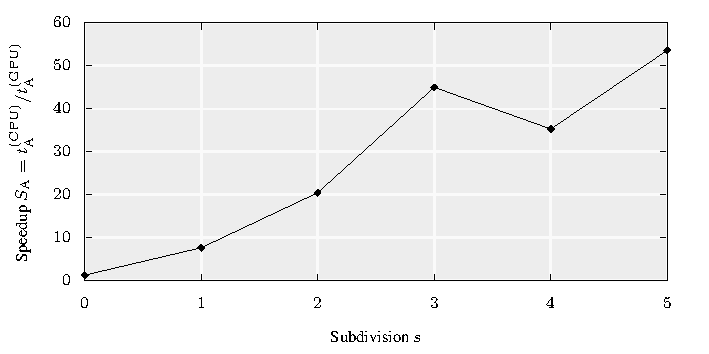
\includegraphics[width=0.95\textwidth]{plots/speedup_plot.pdf}
      \caption{}
      \label{fig:speedup}
    \end{figure}

  % section simulation_und_ergebnisse (end)
\end{document}